\documentclass{article}
\usepackage[utf8]{inputenc}
\title{Lecture 9 Decision  Trees}
\author{wbg231 }
\date{December 2022}
\newcommand{\R}{$\mathbb{R}$}
\newcommand{\B}{$\beta$}
\newcommand{\A}{$\alpha$}
\newcommand{\D}{\Delta}

\newcommand{\avector}[2]{(#1_2,\ldots,#1_{#2})}
\newcommand{\makedef}[2]{$\textbf{#1}$:#2 }
\usepackage{tikz,graphicx,hyperref,amsmath,amsfonts,amscd,amssymb,bm,cite,epsfig,epsf,url}

\begin{document}

\maketitle

\section*{introduction}
\begin{itemize}
\item Decision trees are an inherently non linear type of model
\item they are lso a good way to understand Ensemble  methods. 
\section*{Decision trees}
\item regression trees try to predict a continuous outcome 
\item classification trees try to predict a discrete class.
\item a binary tree has 2 children nodes there are also multi-way trees that have more 
\item each node contains a subset of the data 
\item the data splits created by each node involve only a single feature 
\item for continuous variables the splits are always of the form $x_{i}\leq y$
\item for discrete variables we partition the values into two stets 
\item predictors are made in the leaf nodes 
\subsection*{constructing the tree }
\item our goal is to find the boxes $R_1\dots R_J$ that minimize
 $\Sigma_{j=1}^{J}\Sigma_{i\in R_{j}}(y_i-\hat{y}_{R_{j}})$ subject to 
 complexity constraints 
\item the issue with this is finding the true optimal binary tree is computationally
intractable
\item so instead we use a greedy algorithm  (that is we take the best choice at every step)
where we start at the root and on our first step take the splits that would 
result in the minimal loss, and then pass the data split like that to the next
step and have each for each of those sections pick the best splits
and continue this until we hit some stopping criteria
\item we only split regions defined in the last step at each current step 
we predict based on the mean value of a terminal node ie $\hat{y}_{R_{m}}=mean(y_i|x_i\in R_{m})$ 
\item so building a tree like this we are making the best local choice at every step but are unlikely to reach the overall optimal choice
\item \includegraphics*[width=10cm]{lecture_notes/lecture_9/immages/l9_1.png}
\item so the left is how the tree looks for regression 
\item each node, is a binary decision with a condition that splits the tree remaining data into 2 groups in the binary case 
\item the the right side, is the search space. as you can see node (that is condition) make s a linear subdivision of our search space. 
\item 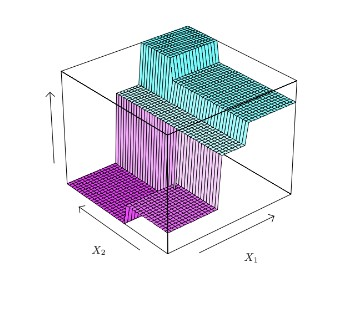
\includegraphics[width=10cm]{lecture_notes/lecture_9/immages/l9_2.jpg}
\item geometrically this looks like this kind of step wise division as can be seen in this chart. 
\subsection*{ finding the best split point}
\item there are infinitely many split points for each feature. 
\item suppose we have a vector $D=\{(x^1,y^1)...(x^n,y^n)\}$ where $x^i\in \mathbb{R}^{d}, y^i\in \mathbb{R}\forall i \in [1,n]$
\item suppose we are not considering splitting on the jth feature. ie $x^{i}_j$ 
\item we can sort our values by there value of the jth feature as $x_{j}(1)\cdots x_j(n)$
\item lets only consider split points between two adjacent values. note that any split point between the two same values will have the same loss.
\item due to this it is common to split half way between the two adjacent values $$s_j\in \{\frac{1}{2}(x_j(r)+x_{j}(r+1)|r=1\cdots n-1\}$$
so this is just saying that geometrically we are taking our split to be halfway between two adjacent points 
\subsection*{decision trees and over fitting}
\item we can keep splitting our data Intel every point has its own region. however doing so would clearly be over fitting
\item so the questions becomes when should we stop splitting a tree? (ie how can we control the complexity of $\mathcal{F}$
\begin{enumerate}
    \item we could limit the total number of nodes
    \item we could limit the number of terminal nodes
    \item we could limit the total depth of the tree 
    \item we could require a certain number of data points be in each terminal node
    \item we could conduct backwards pruning using the CART method 
    \begin{enumerate}
        \item first we build a really tree (ie until all terminal nodes have less than 5 points each)
        \item then we can prune the tree, greedily removing the node at each step that most increases our performance on the validation set, and continue this until validation performance falls.
        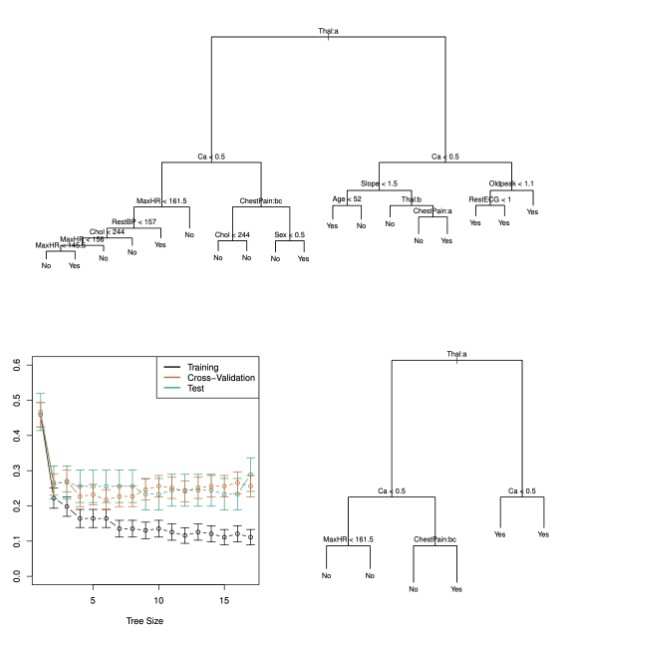
\includegraphics[width=10cm]{lecture_notes/lecture_9/immages/l9_3.jpg}
        \item here is what pruning can look like 
        \item so you can see as tree size goes up (past a certain point) we over fit,
    \end{enumerate}
\end{enumerate}
\subsection*{good splits for classification}
\item in classification we basically want to predict the majority label for each region 
\item we want to produce nodes that have the most instances of the same class (called pure nodes). So that means within each node there should be a lot of one class and not much of any other ideally
\subsection*{Misclassification   error in a node}
\item suppose we are dealing with multi class labels with outputs space $y=\{\1...k\}$
\item let node m represent region $R_{m}$ with $N_m$ observations within it
\item we denote the proportion of observations in $R_M$ with class k by 
$$\hat{\rho}_{mk}=\frac{1}{N_{m}}\Sigma_{i:x_{i}\in R_{m}}\mathbb{I}(y_i=k)$$ 
\item we predict all new data points in node m by the majority class $$\hat{\rho}_{mk}(m):=argmax_{k}\hat{\rho}_{mk}$$
\subsection*{node impurity measures}
\item the purity of a node is how much agreement there is within that node on class
\item three main measures of node impurity for leaf node m  are
\begin{enumerate}
    \item the Misclassification  rate for node m class k is  $$\ell(m):=1-\hat{\rho}_{mk}$$
    \item the gini index $$\ell(m)=\Sigma_{k=1}^{K}\hat{\rho}_{mk}(1-\hat{\rho}_{mk})$$ this encourages our prediction to be close to 0,1. that is it gives over all classes that we could predict, takes the product of the proportion that are class k and there complement and sums them.
    \item finally we have entropy or information gain $$-\Sigma_{k=1}^{K}\hat{\rho}_{mk}log(\hat{\rho}_{mk})=E[-log(\hat{\rho}_{mk})]$$
    this can more or less be thought of as a measure of how predictable a random variable is. so we would like this value to be low \href{https://en.wikipedia.org/wiki/Entropy_(information_theory)}{wiki}
\end{enumerate}
\item the gini index and entropy both work better in practice
\item 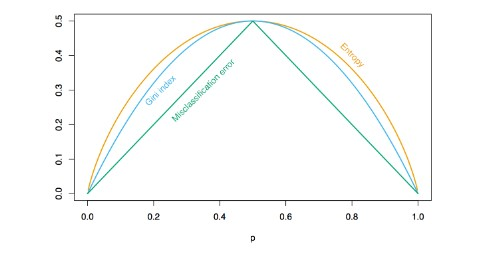
\includegraphics[width=10cm]{lecture_notes/lecture_9/immages/l9_4.jpg}
\item here is what they look like graphed out. we can see that Misclassification rate, is a step-wise  linear function so is more likely to result, in in balanced classes. where as the gini index and entropy are non linear and thus heavily encourage unbalanced classes
\subsection*{quantifying the impurity of a split }
\item suppose we have a split $S_i$ that products nodes $R_L, R_R$ with $N_L, N_R$ points respectively. 
\item let $Q$ be a function that measures node impurity
\item we would call the impurity of this $$\ell(S_i)=\frac{N_L(Q(R_R)+N_R(Q(R_R)}{N_L+N_r}$$ that is the loss or impurity of a split is a weighted average of the impurity of the nodes it produces. 
\subsection* {Interpretability  of decision trees}
\item trees are very easy to visualize and explain 
\item small trees have high  Interpretability large trees not so much. 
\subsection*{tree vs linear model}
\item trees can do a very good job capturing non-linear relationships, but may have a hard time capturing linear ones. 
\item 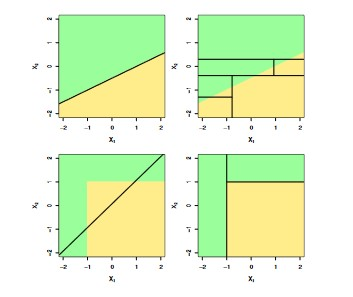
\includegraphics[width=10cm]{lecture_notes/lecture_9/immages/l9_5.jpg}
\item Decision tree models make decisions based on the hierarchy of rules that recursively divide the feature space into smaller regions. Each internal node in the decision tree represents a test on a feature, and each branch represents the outcome of that test. In contrast, linear models try to find the linear relationship between the features and the target variable.

\item While decision trees can capture nonlinear relationships well, they have a hard time capturing linear relationships in the data because they rely on a hierarchical structure of rules to partition the data space, whereas linear models can directly model linear relationships in the data. Decision trees require many splits to represent linear relationships, leading to a tree that is very deep and complex. As a result, decision trees tend to overfit the training data when trying to capture linear relationships, making them less effective than linear models.

\item Linear models, on the other hand, are designed to capture linear relationships in the data by finding the best linear combination of the features that explains the target variable. Linear models can represent complex nonlinear relationships by using nonlinear transformations of the features or by combining multiple linear models. This makes them more effective at capturing linear relationships than decision tree models.
\subsection*{review}
\item trees are 
\begin{itemize}
    \item non linear the decision boundary that results from splitting may end up being quite complicated 
    \item non-metric that is they do not rely on the geometry of input space, they are just binning features
    \item they are non-parametric that is they make no assumptions about the distribution of our data. (contrasted with parametric models like linear models which assume the relationship is distributed lineally) 
\end{itemize}
\item additionally they are Interpretable and easy to understand 
\item they do have the following drawbacks
\begin{enumerate}
    \item they have a hard time capturing linear relationships
    \item they have high variance and tend to overfit. they are sensitive to small changes in the training data 
\end{enumerate}
\section*{bagging and random forests}
\subsection*{point estimators}
\item suppose we have data set $\mathcal{D}=\{x_1..x_n\}$ that was sampled iid from some parametric distributions $P(\cdot|\theta)$
\item a statistic $s=s(\mathcal{D})$ is any function of the data for instance mean variances covariance or entropy
\item $\mathbf{a point estimator}$ of $\theta$ is a statistic $\hat{\theta}=\hat{\theta}(\mathcal{D})$ if $\hat{\theta}\approx \theta$ simply it is just an estimate of a population parameter from data. 
\subsection*{bias and variance of an estimator}
\item let $\hat{\theta}(\mathcal{D})$ be an unbiased estimator with variance $\sigma^2$ 
\item thus we know $E[\hat{\theta}]=\theta$
\item $var(\hat{\theta})=\sigma^2$ meaning that its standard error is $$se(\hat{\theta})=\sqrt{var(\hat{\theta})}=\sigma$$
\item consider  a new estimator that takes the average of n calculations of $\hat{\theta}$ on n iid data sets $\mathcal{D}^1...\mathcal{D}^n$
\item call this new estimator $\hat{\theta}=\frac{1}{n}\Sigma_{i=1}^{n}(\hat{\theta}_{i})=\frac{1}{n}\Sigma_{i=1}^{n}(\hat{\theta}(\mathcal{D}^i))$
\item we can see that $E[\hat{\theta}]=E[\frac{1}{n}\Sigma_{i=1}^{n}\hat_{\theta_i}]=\theta$
\item furhter we can see that $var(\hat{\theta})=E[(\hat{\theta}-E[\hat{\theta}])^2]=E[(\frac{1}{n}\Sigma_{i=1}^{n}\hat_{\theta_i}-E[\frac{1}{n}\Sigma_{i=1}^{n}\hat_{\theta_i}])^2]$ $=E[(\frac{1}{n}(\Sigma_{i=1}^{n}\hat_{\theta_i}-E[\Sigma_{i=1}^{n}\hat_{\theta_i}]))^2]=\frac{1}{n^2}E[(\Sigma_{i=1}^{n}  \hat{\theta}_i -E[\hat{\theta}_i] )^2 ]=\frac{\Sigma_{i=1}^{n}}{n^2}E[(
\hat{\theta}_i -E[\hat{\theta}_i] )^2 ]=\frac{n\cdot var(\theta_{i})}{n^2}=\frac{var(\theta_{i})}{n}=$ $\frac{\sigma^2}{n}$
\item so this all goes to show that the mean of a point estimator that is unbiased, will have the same mean (that is remain unbiased) but have lower variance the more estimations you take
\subsection*{averaging independent prediction functions }
\item suppose that we have $B$ independent training sets all drawn from the same distribution that is $\mathcal{D}_{i}\sim P(\cdot|\theta)\forall i\in [1,b]$
\item our learning algorithm will then produce $B$ prediction  functions $\hat{f}=\{\hat{f}_1(x)\cots \hat{f}_B(x)\}$
\item then we can define the average predication function as $$\hat{f}_{avg}(x):=\frac{1}{B}\Sigma_{b=1}^{B}\hat{f}_{b}(x)$$
\item as we showed above $E[\hat{f}_{avg}(x)]=E[\hat{f}_{i}(x)]\forall i \in [1,b]$
\item but $var(\hat{f}_{avg})=\frac{1}{B}var(\hat{f}_{i}(x))\forall i\in [1,B]$
\item \textbf{there is an issue however, this is all reliant on the fact that we have B independent training sets, which we can not have in practice}
\subsection*{the bootstraps sample}
\item how do we simulate many samples when we only have one?
\begin{enumerate}
    \item we can boostrap
    \item a bootstrap sample from dataset $\mathcal{D}_{n}=(x_1..x_n)$ is a samples of size n drawn with replacement from the dataset 
    \item some elements in our data set will show up multiple times in a given bootstraps others will not show up at all 
    \item each $x_i$ has a pro ability of not being included in a given bootstrap sample at position j as  $P(x_i= B_j)=\frac{1}{n}$ that is the likelihood of any single sample being in the bootstrap B at any given point is uniform. as we are drawing with replacement we know these events will be iid thus the likelihood that $x_i$ will not be in the boot strap at any of the n positions is  $$P(x_i\not \in B)=P(\Cap_{j=1}^{n}x_i\not \in B_j)=1-P(\Cup_{j=1}^{n}x_i\in B_j)=\Pi_{j=1}^{n}1-P(x_i=B_j)$$ 
    $$=(1-P(X_i=B_j))^{n}=(1-\frac{1}{n})^{n}\approx (1+\frac{1}{n})^{-n}=(\frac{1}{e})\approx .368 $$ (given we take n towards infinity)
    \item so in other words for a sample of infinite size, each individual $x_i$ has around a $\frac{2}{3}$ chance of being in each boot strap
\end{enumerate}
\subsection*{the boot strap method}
\item \textbf{bf}{a bootstrap method } simulates $B$ independent samples from P by taking B bootstrap samples from out empirical sample $\mathcal{D}_{n}$
\item given the original data $\mathcal{D}_{n}$ compute b boostrap samples $D_n^1...D_n^b$
\item for each bootstrap sample compute some function $\phi(D_{n}^{1})\dots \phi(D_{n}^{B})$
\item use these values as if there were iid samples from p 
\item this ends up approximating iid samples really well (if our original dataset was good)
\subsection*{ensemble methods}
\item in general ensemble methods combine multiple weak models into a single more power full model
\item averaging iid estimates reduces our variance with out changing the bias 
\item we can bootstrap to simulate multiple data sample sand average them 
\item we can either use parallel ensemble methods like bagging when models are built independently
\itme or we can use sequential ensemble methods where models are built sequentially

\subsection*{Bagging: boostrap aggregation}
\item we draw $B$ boot strap samples $D^1...D^n$ from original data $\mathcal{D}$
\item learn the corresponding prediction functions  $\hat{f}_1\cdots \hat{f}_n$
\item and define the bagged prediction function as a combination of these $\hat{f}_{avg}(x)=combine(\hat{f}_1\cdots \hat{f}_n)$
\item bagging is a general model that works really well on trees
\item for classifications we can combine predictors by taking a majority vote
\item increasing the number of trees we use in bagging does not lead to over fitting 
\item the down side is that bagged trees are a lot less interpretable than single decision trees
\subsection*{out of bag estimation }
\item recall that each bagged predictor is trained on about 66\% of the training data 
\item the remaining 37\% are called the out of bag (OOB) observations 
\item so let $S_i=\{x_i|x_i\not \in D^{b}\}$
\item the oob prediction on $x_i$ is $$\hat{f}_{oob}(x_i)=\frac{1}{||S_i||}\Sigma_{b\in S_i}\hat{f}_{b}(x_i)$$
\item the oob error can be used to gauge test error in a way that is similar to Cross validation 
\item bagging will do well when each of the base learners is unbiased (or nearly) and have high variance
\subsection*{motivating random forests: correlated prediction functions}
\item everything we have done with bagging is based off the assumption that our bootstraps are iid
\item so note that boot strap samples are independent samples from the training set but are \textbf{not independent samples from the population distribution}
\item this means that there will be correlation between predictors that are estimated on different bootstraps
\item given this is the case we still have $E[\frac{1}{n}\Sigma_{i=1}^{n}\hat{\theta}_i]=\mu$ 
\item however $var(\frac{1}{n}\Sigma_{i=1}^{n}\hat{\theta_i}=cov(\frac{1}{n}\Sigma_{i=1}^{n}\theta_i,\frac{1}{n}\Sigma_{j=1}^{n}\theta_j)=\frac{1}{n^2}cov(\Sigma_{i=1}^{n}\theta_i,\Sigma_{j=1}^{n}\theta_j)=\Sigma_{i=1}^{n}\Sigma_{j=1}^{n}\frac{1}{n^2}cov(\theta_i,\theta_j)=\frac{1}{n}^2(\Sigma_{i=1}^{n}var(\theta_i)+\Sigma_{j\geq i}cov(\theta_i, \theta_j)=\frac{\sigma^2}{n}+\frac{1}{n^2}\Sigma_{i=1}^{n}\Sigma_{j\geq i}cov(\theta_i, \theta_j)$
\item so notice in this case there will be n variance terms and $\begin{pmatrix}n\\2\end{pmatrix}$ covariance terms (which will each be multiplied by 2). thus as n grows the covariance term will dominate the variance  of our bagged estimator, causing the benefits of averaging to fall
\subsection*{random forests}
\item the key idea here is that we are slightly modifying bagging to reduce the dependence between trees 
\item we do this by 
\begin{enumerate}
    \item building a collection of trees in parallel as before
    \item when constructing each tree node restrict the choice of the splitting variable to a randomly chosen subset of features of size  (that is only allow that tree to learn about m out of the total d features)
    \item this prevents the situation where all trees are dominated by a small number of strong features (highly predictive) and thus are to similar to one another 
    \item we typically chose $m\approx \sqrt{d}$ where d is the number of features 
    \item if m=p then we have typical bagging 
\end{enumerate}
\item note that this does not completely prevent correlation between trees it just lowers it 
\item empirically this procedure does well
\subsection*{ review}
\item the usual approach is to build very deep trees with low bias and high variance
\item ensemble models reduce variance but remain unbiased 
\item use a bootstrap to simulate many data samples form one dataset 
\item but bootstrap samples and the point estimators they produce are correlated
\item so we use random forests and teach each tree only on a random subset of the features as ensemble methods work better on diverse set of prediction functions 

\section*{boosting}
\subsection*{overview}
\item bagging try to reduce variance of a low bias high variance estimator by ensemble many estimator trained in parallel on different boots rap samples of our dataset.
\item boosting reduces the error rate of a high bias estimator by ensembles many estimators trained in sequence 
\item like bagging boosting is a general method that is popular with trees 
\item the general idea is that instead of fitting the data very closely using a large decision tree, we train gradually using a sequence of simple trees
\subsection*{boosting overview}
\item \textbf{a weak or base learner} is a classifier that does slightly better than chance
\item weak learners are kind of like rules of thumb, they learn rules like if a word is present that means an email is spam or if you get an email form a friend it will not be spam 
\item the key ideas are that each weak learner focuses on different training examples by re-weighting the data, and each weak learner makes different contributions to the final predictor
\item a set of smaller more simple trees may make things more improve interpretability
\item we will focus on the ada boost implementation
\subsection{ada boost setting}
\item output space $Y=\{-1,1\}$ ie binary classification 
\item base hypothesis space $\mathcal{H}=\{h:X\rightarrow \{-1,1\}\}$ that is functions mapping from our input space to the output space 
\item typical base hypothesis spaces are 
\begin{enumerate}
    \item \textbf{decision stumps} where each tree has only a single split 
    \item trees with few terminal nodes
    \item linear decision functions 
\end{enumerate}
\subsection{weighted training set}
\item each base learner is trained on weighted data 
\item let the training set be $\mathcal{D}=((x_1,y_1)...(x_n,y_n))$
\item and further let there be weights $(w_1...w_n)$ associated with each example
\item thus we define \textbf{ the weighted empirical risk} as $$\hat{R}_{n}^w:=\frac{1}{W}\Sigma_{i=1}^{n}w_i\ell(f(x_i),y_i) \text{ where } W=\Sigma_{i=1}^{n}w_i$$
\item so as you would exact is a weighted sum of our loss function. 
\item we learn classifiers $G_{i}(x)\forall i\in [1,M]$ and take our final classifier as $G(x)=sign[\Sigma_{m=1}^{M}\alpha_{m}G_m(x)]$ 
\subsection*{ada boost sketch}
\item start with equal weights of training points $w_1=..=w_n=1$
\item repeat for m=1..M where M is the number of classifiers we want to train 
\begin{enumerate}
    \item train base classifier $G_m(x)$ on the weighted training data. this classifier may not fit the data well
    \item increase the weight of the points missclassifed by $G_m(X)$
\end{enumerate}
\item our final predictor is $G(x)=sign[\Sigma_{m=1}^{M}\alpha_{m}G_m(x)]$ 
\item we would like $\alpha_{m}$ to be non negative and larger when $G_m$ fits its weighted training data well
\item the weighted zero one error of $G_m(X)$ is $$err_{m}=\frac{1}{W}w_i\mathbb{I}(y_i\neq G_m(x_i)) \text{   where } w=\Sigma_{i=1}^{n}w_i$$that is basically the weighted average of the number of points each classifier gets right 
\item then we can say that the weight of classifier $G_{m}(x)$ is $\alpha_{m}=ln(\frac{1-err_m}{err_m})$
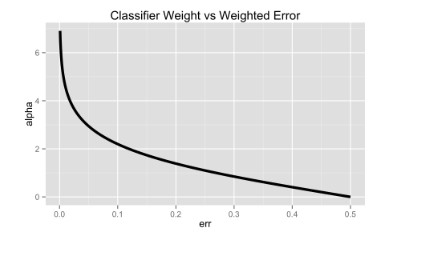
\includegraphics[width=10cm]{lecture_notes/lecture_9/immages/l9_6.jpg}
\item where higher weighted error implies lower wight on that classifier
\subsection{example}
\item suppose we train classifier $G_m$ to minimize weighted error, which results in error rate $err_m$
\item then the classifier weight of $G_m$ in the final ensemble is $\alpha_m=ln(\frac{1-err_m}{err_m})$
\item we want the next base learner $G_{m+1}$ to focus on the examples that $G_m$ messed up 
\item suppose $w_i$ is the weight of example $x_i$ before training $G_m$
\begin{itemize}
    \item if $G_m$ get $x_i$ correctly keep $w_i$ the same
    \item otherwise increase $w_i$ such that $w_i\leftarrow w_ie^{\alpha_m}=w_i(\frac{1-err_m}{err_m})$
    \item if $G_m$ is a Strong classifier overall then $\alpha_m$ will be large and misscalsied points will have much larger weights. 
\end{itemize}
\subsection{ada boost algorithm}
\item given training set $\mathcal{D}=\{(x_1,y_1)\cdots (x_n,y_n)\}$
\begin{enumerate}
    \item initialize observation weights $w_i=1$ for all i 
    \item for m=1 to M (number of trees we want to train) 
    \begin{itemize}
        \item base learner fits the training data and returns $G_M(x)$
        \item compute the weighted empirical 0-1 risk $$err_{m}=\frac{1}{W}w_i\mathbb{I}(y_i\neq G_m(x_i)) \text{   where } w=\Sigma_{i=1}^{n}w_i$$
        \item compute the classifier weight $\alpha_m=ln(\frac{1-err_m}{err_m}$
        \item update the example weight $w_i\leftarrow w_i \cdot e^{\alpha_m \mathbb{I}(y_i\neq G_m(x_i))}$
    \end{itemize}
    \item return final classifier $G(X)=sign[\Sigma_{m=1}^{m}\alpha_m G_m(x)]$
\end{enumerate}
\subsection{ada boost over fitting}
\item does a large number of boosting lead to over fitting?
\item no not really since we are learning week learners, we should be resilient to over fitting 
 
\end{itemize}
\end{document}
